\documentclass[11pt]{article}
\usepackage[T1]{fontenc}
\usepackage[utf8]{inputenc}
\usepackage[french]{babel}
\usepackage[a4paper]{geometry}
\usepackage{color}
\usepackage{changepage}
\usepackage{float}
\usepackage{amsmath}
\usepackage[hidelinks]{hyperref}
\usepackage{graphicx}
\usepackage{array}


\begin{document}
\begin{figure}
    
\includegraphics[height=1cm]{logolemansU.png}
    \hfill
    
\includegraphics[height=1cm]{logo_IC2.png}
\end{figure}
    \title { 
        \textcolor{blue}{Le Mans Université} \\
        \texttt{Licence Informatique 2ème année} \\
        \texttt{Module 174UP02 Rapport de projet}\\
        \textbf{VoidBorn}\\
        \href{https://github.com/Herebios/projet}{Lien vers le Github}
    }
    
    \author{Baptiste M, Lucas R, Nathan M, Ilann T} 
    \date{\today} 
    \maketitle

    \newpage
    \tableofcontents
    \newpage
    
    \section{Introduction}
    Nous sommes un groupe de quatre étudiants à l’Université du Mans. Notre objectif a été de créer un jeu en respectant un délai d’environ trois mois.
    Lors de notre phase de réflexion, nous souhaitions créer un jeu multijoueur en deux dimensions à l’aide de la bibliothèque graphique SDL2, en langage C.
    Pendant une partie, deux équipes s’affrontent pour détruire la base adverse tout en protégeant la leur.
    Nous nous sommes fixé comme contrainte de développer ce jeu en réseau.

    \section{Analyse}
    Dans le menu, chaque joueur choisit son pseudo ainsi que la classe de son personnage, ce qui lui confère des capacités uniques qu’il peut utiliser au cours de la partie pour prendre l’avantage sur l’équipe adverse.
    Vous avez alors le choix entre être le serveur de la partie, être joueur d’une partie ou être les deux à la fois. \\
    Après cela, vous arrivez dans une salle d’attente, en attendant que les autres joueurs se joignent à vous. Une fois que la personne jouant le rôle de serveur lance la partie, le jeu démarre. \\
    La map de notre jeu se décompose en plusieurs zones que nous appelons tuiles, chacune ayant un biome(neige, plaine, etc) choisi aléatoirement. \\
    Les joueurs ne peuvent visualiser qu’une tuile du jeu à la fois. Cependant, il est possible de changer de tuile en passant par des portes placées à différents endroits 
    aux bords de la tuile à la manière de \href{https://en.wikipedia.org/wiki/The_Binding_of_Isaac_(video_game)}{The Binding of Isaac}. \\
    Des obstacles sont générés aléatoirement sur la map, limitant les déplacements des joueurs. \\
    Des monstres sont également présents sur la map, se dirigeant vers le joueur le plus proche pour l’attaquer. Lorsque le monstre est tué il lâche un objet que le joueur peut
    ramasser et ajouter à son inventaire.\\
    Chaque objet a une rareté et confère au joueur différents effets. Plus la rareté de l’objet est élevée, plus les effets bonus conférés au joueur sont importants. \\
    Un système de combat est mis en place entre les joueurs d’équipes différentes lorsqu’ils se trouvent sur la même tuile. \\
    Les points de vie ainsi que les objets du joueur sont affichés sur son écran à la manière d’un inventaire \href{https://fr.wikipedia.org/wiki/Minecraft}{Minecraft}.\\ 
    La gestion des entités dynamiques et des tuiles de la map est réalisée grâce à l’implémentation d’une liste générique. 
    Le serveur communique avec les clients en envoyant toutes les informations nécessaires à l’affichage du jeu par le client qui renvoie des informations au serveur 
    en fonction des actions du joueur.
    
    \section{Organisation du Projet}
    Le groupe a organisé le travail autour de différents outils pour contrôler l’avancement du projet. Le dépôt git sert à stocker les fichiers. Un document partagé Google Drive a servi à noter les idées au lancement du projet et à préparer le compte-rendu. Puis, l’application Trello et un diagramme de Gantt nous ont permis de répartir les tâches efficacement au cours du temps.

        \subsection{Planning Prévisionnel}
        Ci-dessous notre planning prévisionnel sur 3 mois. (Voir Figure~\ref{fig:Gant})
        \begin{figure}[H]
            \begin{center}
                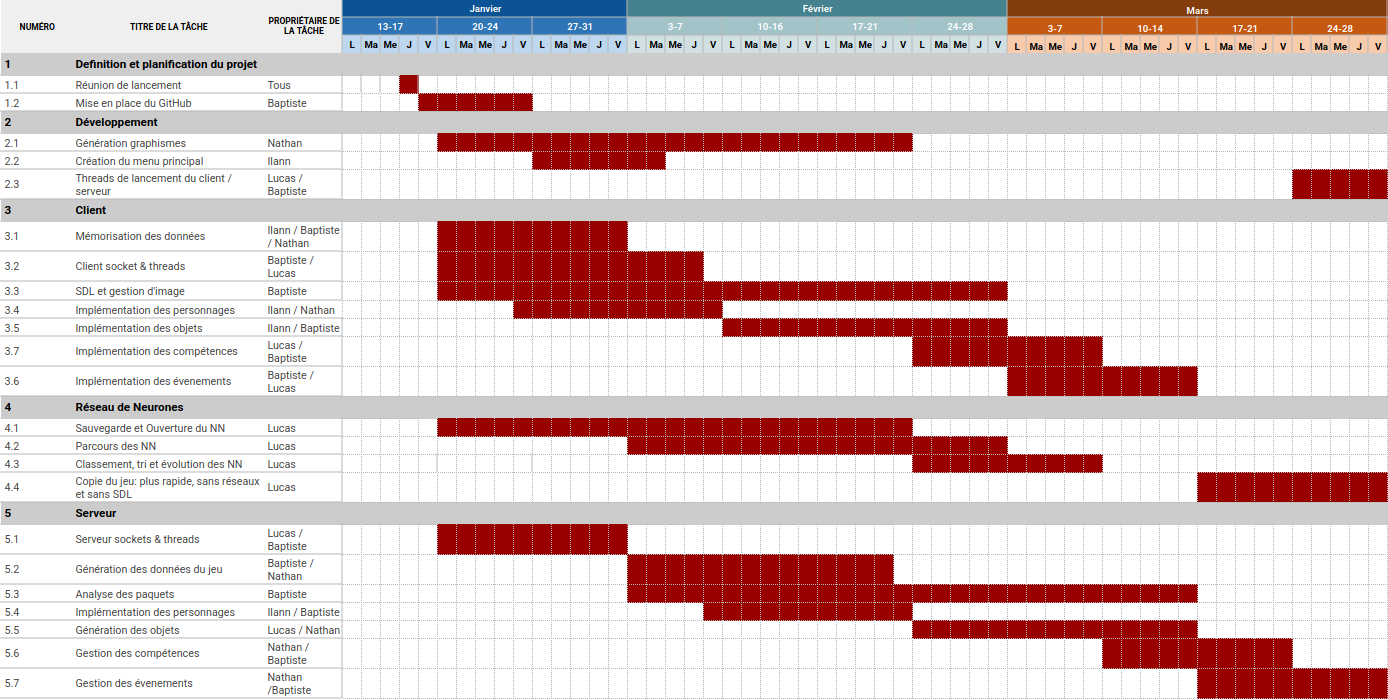
\includegraphics[height=9cm]{gant.png}
                \caption{Diagramme Gant}
                \label{fig:Gant} 
            \end{center}
        \end{figure}
        \subsection{Répartition des tâches}


        Nous nous sommes répartis les tâches de la manière suivante :
        \begin{itemize}
            \item Baptiste : affichage du client, déplacement d’un personnage, gestion de la carte et des tuiles. Réalisation de la partie réseau, de l’envoi des informations au lancement du jeu, le format des messages, la mémorisation et le traitement des informations du jeu pour le client et le serveur.       
            \item Lucas : réalisation du réseau de neurones, une partie qu'il n’est pas possible de rattacher au jeu dans son état actuel. Lucas a aussi sa part dans la partie réseaux avec la création de la file et la mise en place des threads et de l’écoute des flux. Les compétences ont aussi été développées, dans l’état l’implémentation n’est pas concluante et ne peut pas être ajoutée au jeu. Résolution de nombreux bugs dans tout le projet. 
            \item Ilann : réalisation du menu, dans le but de récupérer le pseudo, le personnage ainsi que l'adresse IP d’un joueur ou serveur. Réalisation de l’affichage des objets dans l’inventaire des joueurs ainsi que leur récupération sur la carte et la possibilité de les relâcher.  
            \item Nathan : réalisation des statistiques des personnages, création des objets permettant la modification des statistiques du joueur et implémentation des monstres (partiellement intégrés au jeu). Génération de beaucoup d'images et de textures de la map, laissant une liberté de choix graphique.
        \end{itemize}
    \section{Développement}
    Cette partie abordera le développement du jeu dans sa globalité. De la création des ressources graphiques à la création du client/serveur en passant par la gestion de la carte, des objets, etc. 
        \subsection{Création des ressources}
        Cette section abordera la génération des ressources graphiques de base permettant la réalisation du jeu.
            \subsubsection{Objet}
            Quarante objets sont présents dans le jeu. Tous sont générés avec un prompt chatGPT.\\
            Quelques exemples d'objets ci-dessous (Figure~\ref{fig:BagueMageNoir}, Figure~\ref{fig:OrbeMystique}).
            \begin{figure}[H]
                \centering
                % Première image
                \begin{minipage}{0.45\textwidth}
                    \centering
                    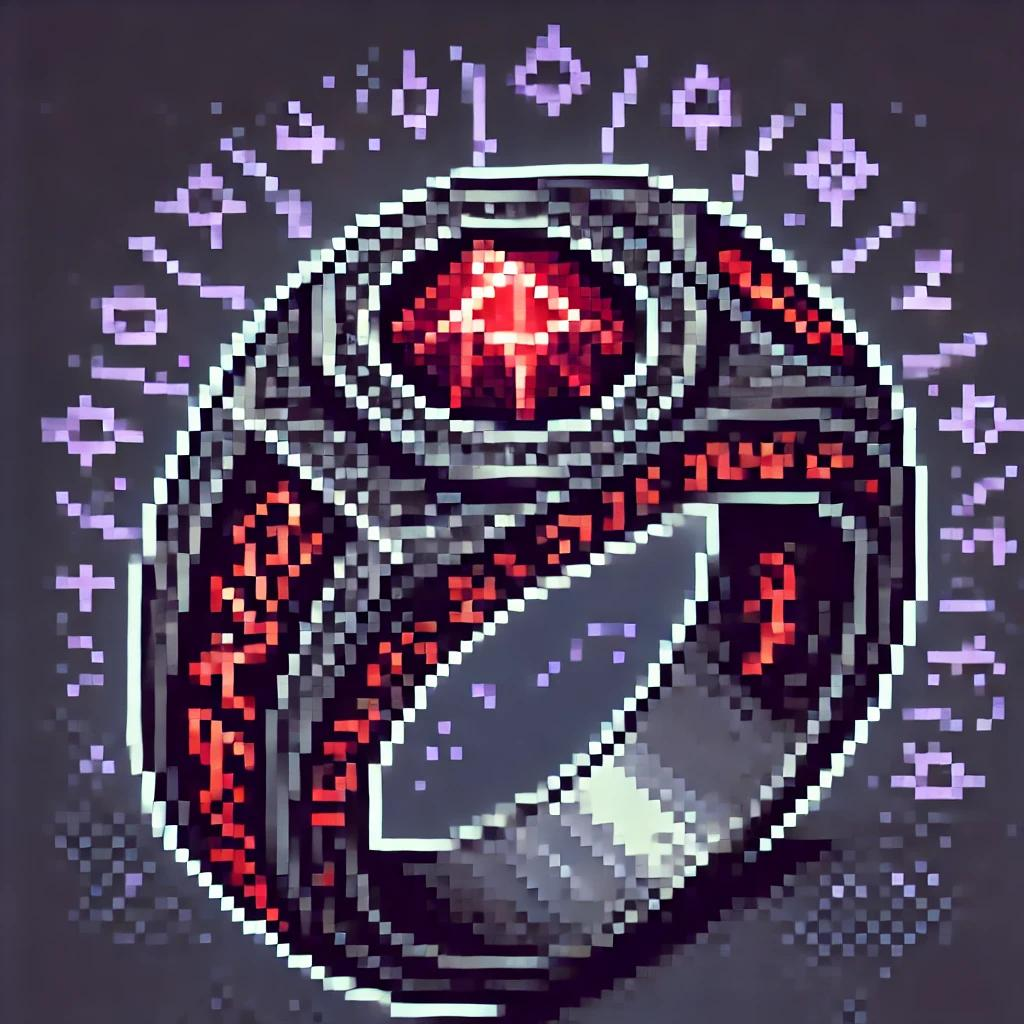
\includegraphics[height=4cm]{Bague du mage noir.jpg}
                    \caption{Bague du mage noir}
                    \label{fig:BagueMageNoir}
                \end{minipage}
                \hfill
                % Deuxième image
                \begin{minipage}{0.45\textwidth}
                    \centering
                    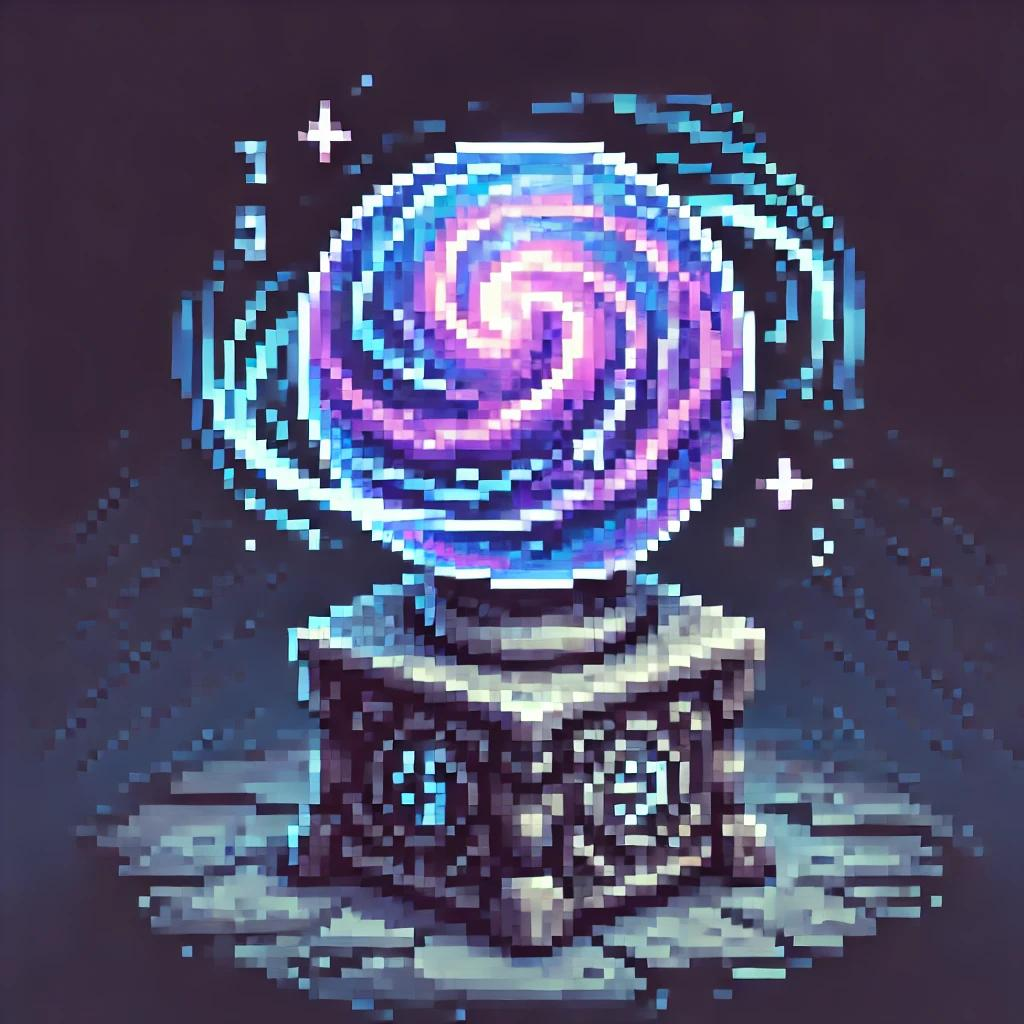
\includegraphics[height=4cm]{Orbe mystique.jpg}
                    \caption{Orbe mystique}
                    \label{fig:OrbeMystique}
                \end{minipage}
            \end{figure}
            \subsubsection{Sprites et Personnages}
            Quatre personnages sont présents dans le jeu :
            \begin{itemize}
                \item Archer
                \item Mage
                \item Ninja
                \item Vampire
            \end{itemize}
            Chaque personnage a un spritesheet de 12 images (3 images par direction).\\
            Quelques exemples de spritesheet ci-dessous (Figure~\ref{fig:Mage}, Figure~\ref{fig:Archer}). 
            \begin{figure}[H]
                \centering
                % Première image
                \begin{minipage}{0.45\textwidth}
                    \centering
                    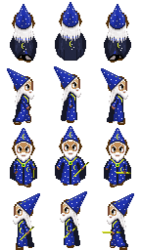
\includegraphics[height=4cm]{mageSrc.png}
                    \caption{spritesheet Mage}
                    \label{fig:Mage}
                \end{minipage}
                \hfill
                % Deuxième image
                \begin{minipage}{0.45\textwidth}
                    \centering
                    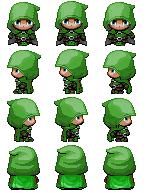
\includegraphics[height=4cm]{archerSRC.png}
                    \caption{spritesheet Archer}
                    \label{fig:Archer}
                \end{minipage}
            \end{figure}
            \subsubsection{Tuiles et Biomes}
            Six biomes différents sont implémentés dans le jeu.\\
            Chaque biome a :
            \begin{itemize}
                \item une texture de base pour le sol (voir Figure~\ref{fig:normal})
                \item une texture pour un premier obstacle (voir Figure~\ref{fig:obstacle1})
                \item une texture pour un deuxième obstacle (voir Figure~\ref{fig:obstacle2})
                \item une texture pour indiquer la sortie d'une tuile (voir Figure~\ref{fig:sortie})
            \end{itemize}
            Voici un exemple des quatre textures du biome plaine ci-dessous. 
            \begin{figure}[H]
                \centering
                % Première image
                \begin{minipage}{0.45\textwidth}
                    \centering
                    
\includegraphics[height=1.5cm]{normal.png}
                    \caption{Texture base}
                    \label{fig:normal}
                \end{minipage}
                \hfill
                % Deuxième image
                \begin{minipage}{0.45\textwidth}
                    \centering
                    
\includegraphics[height=1.5cm]{obstacle1.png}
                    \caption{Texture obstacle1}
                    \label{fig:obstacle1}
                \end{minipage}
            \end{figure}
            \begin{figure}[H]
                \centering
                % Troisième image
                \begin{minipage}{0.45\textwidth}
                    \centering
                    
\includegraphics[height=1.5cm]{obstacle2.png}
                    \caption{Texture obstacle2}
                    \label{fig:obstacle2}
                \end{minipage}
                \hfill
                % Quatrième image
                \begin{minipage}{0.45\textwidth}
                    \centering
                    
\includegraphics[height=1.5cm]{sortie.png}
                    \caption{Texture sortie}
                    \label{fig:sortie}
                \end{minipage}
            \end{figure}

        \subsection{Implémentation}
        Nous allons maintenant présenter les différentes structures de données mises en œuvre pour la réalisation du jeu.
            \subsubsection{Map}
            La map est inspirée des jeux comme \href{https://en.wikipedia.org/wiki/The_Binding_of_Isaac_(video_game)}{The Binding of Isaac}, 
            dans lesquels le joueur se déplace de salle en salle dans les quatre directions. \\
            On appelle ces salles des tuiles. De plus, la map est constituée de différents biomes qui déterminent l'apparence de la tuile. Similaires aux biomes de \href{https://fr.wikipedia.org/wiki/Minecraft}{Minecraft},
            les textures diffèrent selon les biomes (forêt, plaine, montagne, désert, neige, glace).
            Pour que le jeu soit rejouable et intéressant, la map est générée procéduralement, en associant à chaque tuile un biome, 
            puis en créant les tuiles en plaçant les textures selon le biome choisi.\\
            Dans le programme écrit en C, la map est une matrice de tuile. Chaque tuile est une structure, qui contient l'information du biome, 
            une matrice des textures qui la composent et les éléments du jeu qui y sont associés.
            On représente les informations par des listes car elles sont variables au cours du jeu et selon les tuiles. 
            Quatre listes tiennent compte des joueurs, des objets, des monstres, et des effets des compétences actives afin de les afficher.
            \subsubsection{Personnages}
            Les personnages sont choisis par les joueurs au début de la partie. Ils sont caractérisés par une classe, comme dans certains jeux de rôle. 
            Cette classe détermine les statistiques de base du personnage et les compétences accessibles. Les statistiques sont la vie, la force, la magie et la vitesse. 
            Chaque personnage a un point fort qui le distingue des autres.\\
            Le personnage est représenté par une structure C. Ses statistiques sont stockées dans deux tableaux de quatre valeurs, 
            ne pour sauvegarder ses statistiques de base et l'autre pour avoir accès à ses statistiques améliorées par les objets. 
            Un tableau de pointeurs permet de retrouver les objets possédés par le joueur.\\
            La fonction creer\_perso permet d’initialiser un joueur à partir de la classe choisie.
            Celle pour le détruire est appelée à la fin du programme.\\
            Pour gérer le déplacement des joueurs, on utilise SDL qui écoute les évènements du clavier. 
            En utilisant l’état des flèches directionnelles, on peut faire changer la direction du joueur avec changer\_dir. 
            Puis la fonction avancer est appelée et change la position du personnage grâce à sa vitesse et sa direction en vérifiant qu’il ne dépasse pas les bords de la tuile. 
            Pour simplifier le calcul, on utilise une table de hachage qui donne une structure qui est le multiplicateur de la vitesse en x et en y selon la direction. \\\\
            \textit{
                Exemple : le joueur se déplace vers le haut et vers la droite, information convertie en une valeur énumérée (type enum en C). \\
                Cette valeur donne un indice pour le tableau deplacement. Le point (0, 0) de la fenêtre est le coin en haut à gauche. La valeur qui correspond à cette direction est la structure de valeurs $x=1$ et $y=-1$, 
                car un déplacement vers la droite signifie ajouter une valeur x (la vitesse du joueur) 
                et un déplacement vers le haut implique de diminuer la valeur y du joueur de sa vitesse aussi.
            }
            \subsubsection{Compétences}
            Les compétences sont les capacités des personnages, elles peuvent être de simples attaques, des techniques de déplacement ou bien des sorts.\\\\
            Elles sont définies de manière statique dans un tableau de structures compétence et de manière dynamique avec la structure \textit{cast}. Quand une compétence est lancée, une structure de \textit{cast} est créée et ajoutée dans une liste. Le \textit{cast} va évoluer en fonction des appels de la fonction \textit{update}. Par exemple, une compétence de zone est supprimée de la liste à la fin de sa durée de vie. La fonction d’update permet aussi de détecter des joueurs en collision pour leur infliger des dégâts ou un autre effet. Les \textit{casts} de compétences sont génériques, on peut ainsi avoir plusieurs types de compétences différentes.\\\\
            L’implémentation des \textit{casts} est différente entre le côté client et le côté serveur.\\
            Le client, au moment de la détection d’une touche d’envoi de compétence, fait une requête au serveur avec les paramètres nécessaires.\\
            Le serveur ajoute ce nouveau \textit{cast} dans une liste et communique avec les joueurs sur la tuile les informations comme la position, la taille pour zone, la portée pour un projectile, etc.
            Le serveur va souvent faire l’update des \textit{casts}, et ainsi envoyer les informations aux joueurs.\\
            Le client, à la suite de la requête du lancement de la compétence s’occupe seulement de la récupération des informations envoyées par le serveur et de l’affichage de la compétence.
            
            \subsubsection{Objets}
            Les objets sont essentiels au jeu. Ils permettent d'augmenter les statistiques de base de notre personnage. 
            Quarante objets sont présents dans le jeu, séparés en quatre catégories de rareté : 
            \begin{itemize}
                \item commun
                \item rare
                \item épique
                \item légendaire
            \end{itemize}
            Chaque objet a quatre statistiques différentes, correspondant à celles d'un personnage :
            \begin{itemize}
                \item vie
                \item force
                \item magie
                \item vitesse
            \end{itemize}
            Ensuite, pour calculer le bonus apporté au joueur par l'objet on différencie trois cas de figure :
            \begin{itemize}
                \item aucun bonus
                \item bonus à additionner 
                \item bonus à multiplier
            \end{itemize}
            Pour garder une certaine cohérence dans les calculs de statistiques du personnage un ordre de calcul a été décidé.
            On effectue d'abord les calculs de somme puis les calculs de produit. Pour ce faire, chaque statistique de l'objet a un couple de valeurs. 
            La première valeur correspond à ce qui est à sommer ou multiplier avec la statistique de base du personnage. 
            La deuxième valeur est un ordre de priorité permettant d'effectuer les calculs dans le bon ordre.
            \\
            \\
            \textit{
                Exemple : si un personnage a deux objets :
                \begin{itemize}
                    \item 1\textsuperscript{er} objet :\{\{0, null\}, \{10, add\}, \{0, null\}, \{-2, add\}\}
                    \item 2\textsuperscript{e} objet : \{\{1.5, mult\}, \{0.8, mult\}, \{20, add\}, \{0, null\}\}
                \end{itemize} 
                On rappelle que les statistiques sont de la forme \{vie, force, magie, vitesse\}.
                Dans cet exemple, on commencera par calculer les trois additions puis les deux multiplications 
                (la somme étant représentée par «add» et le produit par «mult»).
            }\\\\
            Deux fonctions permettent de gérer les objets possédés par le joueur.
            La fonction ajouter\_objet permet de placer un nouvel objet dans l’inventaire à une place libre. La fonction retirer\_objet supprime l’objet à la position donnée.
            Ces fonctions sont appelées par des fonctions de plus haut niveau qui vérifient la présence d’un objet au sol et retirent ou ajoutent l’objet correspondant sur la tuile en fonction de l’action du joueur.

            La fonction update\_stats est appelée quand un joueur gagne ou perd un objet. Elle permet de recalculer les statistiques du personnage

            \subsubsection{Monstres}
            Le jeu intègre des personnages non-joueurs.
            Ce sont des monstres, appelés mobs. Lorsqu'ils sont tués il permettent d'obtenir des objets qui augmentent les capacités de base de notre personnage.
            Les mobs ont plusieurs fonctionnalités. La première est qu'ils se rapprochent du joueur le plus proche à l'aide d'une fonction de calcul de distance.
            \\
            Une fois que cette distance est calculée, la direction que le mob doit prendre est choisie avec un calcul d'angle. 
            Un vecteur horizontal orienté à droite qui servira de base est créé ainsi qu'un vecteur représentant la direction du personnage vers le mob. (Voir Figure~\ref{fig:Mob}) 
            On calcule la valeur en radians de l'angle formé par ces deux vecteurs.\\
            On obtient donc une valeur du cercle trigonométrique que l'on exploite de la manière suivante : 
            \begin{itemize}
                \item Le monstre va en haut si   $ \frac{\pi}{4}  \leq \text{angle} < \frac{3\pi}{4} $
                \item Le monstre va a gauche si  $ \frac{3\pi}{4} \leq \text{angle} < \frac{5\pi}{4} $
                \item Le monstre va en bas si    $ \frac{5\pi}{4} \leq \text{angle} < \frac{7\pi}{4} $
                \item Le monstre va a droite si  $ \frac{-\pi}{4} \leq \text{angle} < \frac{\pi}{4} $
            \end{itemize}

            \begin{figure}[H]
                \centering
                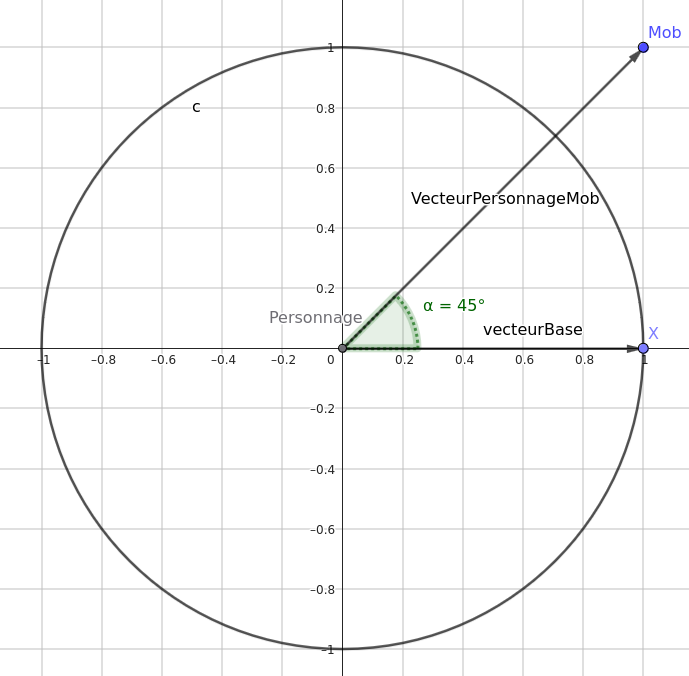
\includegraphics[height=9cm]{cercleTrigo.png}
                \caption{Représentation d'un calcul d'angle en fonction de la position d'un personnage et d'un mob}
                \label{fig:Mob}
            \end{figure}

        \subsection{Réseau}
        Nous allons maintenant voir comment connecter les joueurs avec un serveur pour permettre la connexion et le jeu.
	    Tout d’abord la communication à travers le réseau se fait par des écoutes et des envois dans différents flux. 
        Le client n’a donc comme flux que celui du serveur. Le serveur a bien plus de flux, un pour chaque joueur. 
        La parallélisation est donc obligatoire.

            \subsubsection{Networking}
            Tout d’abord le client se connecte au serveur, suite au choix réalisé dans le menu et à l’initialisation du serveur. \\
            L’envoi et la réception de données s’assurent avec deux fonctions principales :
            La fonction send (qui n’est pas bloquante) permet l’envoi d’un paquet en unicast.
            La fonction recv (qui est bloquante) permet l’écoute du flux et la réception des paquets.
            \\
            La propriété bloquante de recv force l’utilisation de threads.
            Ainsi dès la première connexion, une fonction parallèle d’écoute est créée.
            Le programme possède donc à ce moment :
            \begin{itemize}
                \item Le programme principal qui a appelé la création des autres threads.
                \item Un (ou plusieurs pour le serveur) thread(s) d’écoute. 
            \end{itemize}
            La connexion entre eux se fait par une file. Les threads d’écoute enfilent et le programme principal défile les informations reçues. 
            Les informations sont envoyées d'un côté, passent du thread d’écoute au programme principal de l'autre côté pour ensuite être traitées. \\
            Cette file permet aussi au serveur de traiter les différents clients.\\\\
            Différents codes peuvent être utilisés lors de l’envoi de paquets (Voir Table~\ref{tab:tabCliServ}): 
    
            \begin{table}[h]
                \centering
                \begin{tabular}{|c|c|c|}
                    \hline
                    Code & Nom & Catégorie \\
                    \hline
                    11 & JOUEUR\_CHANGE\_DIR & Joueur \\
                    12 & JOUEUR\_MV & Joueur \\
                    13 & JOUEUR\_MV\_TUILES & Joueur \\
                    ... & ... & ... \\
                    20 & ADD\_OBJET & Objet \\
                    21 & RM\_OBJET & Objet \\
                    ... & ... & ... \\
                    301 & UPDATE\_ZONE & Compétence de zone \\
                    302 & RM\_ZONE & Compétence de zone \\
                    ... & ... & ... \\
                    \hline
                \end{tabular}
                \caption{Différents codes d'action entre le client et le serveur}
                \label{tab:tabCliServ}
            \end{table}

            \subsubsection{Client}
            Au début du jeu, le client se connecte au serveur via socket. Il envoie les informations de son personnage au serveur, puis récupère celles de tous les autres joueurs grâce à lui. Il initialise le jeu grâce aux fonctions \textit{init\_sdl} et \textit{init\_jeu} qui créent respectivement la fenêtre du jeu et les ressources pour la gestion de la map.\\\\
            L’élément principal du programme du client est la boucle de jeu, qui récupère les actions effectuées par le client grâce à SDL. Le joueur se déplace, récupère un objet ou lance une compétence.\\
            Puis, en récupérant un à un dans un buffer les messages stockés dans la file qui écoute le réseau, le client traite les informations qu’il reçoit du serveur. 
            Il récupère de cette manière la position des autres joueurs, leurs actions, s’il doit les afficher, l’ajout et la suppression d’objets sur la tuile, le changement de tuile, etc.
            La fonction \textit{sscanf} de la bibliothèque standard a été très utile pour ça, ainsi que \textit{data\_skip}, écrite pour faciliter la lecture des données dans le buffer.\\\\
            Ensuite le client informe le serveur de ses actions comme un changement de direction, l’utilisation d’une compétence, un objet équipé ou lâché.
            Pour cela, la fonction \textit{sendf} qui utilise \textit{send} inspirée de \textit{sprintf} est utilisée pour mettre en forme les informations à envoyer au serveur.\\\\
            Enfin, le client affiche l’état du jeu. Pour cela, des fonctions s’occupent de charger et d’afficher la tuile courante du joueur. Grâce aux listes actualisées des entités, le client affiche les textures correspondant à tous les personnages, objets et compétences utilisées.

            \subsubsection{Serveur}
            Le serveur est le premier qui démarre, puis se met en attente des joueurs. Une fois tous les joueurs connectés, il envoie un message start avec une graine de génération de la carte. Une fois la partie commencée, le serveur communique les informations sur le jeu à chaque joueur. C’est à ce moment que le serveur se met en écoute, pour gérer la communication entre les joueurs et le jeu de manière générale.\\\\
            Le serveur fonctionne grâce à une boucle dans laquelle il traite les événements arrivant dans le jeu. A partir de cela, il peut modifier les informations du jeu qu’il possède, pour ensuite les communiquer avec les clients. Les informations sont récupérées par une file partagée entre plusieurs threads d’écoutes pour pouvoir écouter chaque client.
            Par exemple, le serveur vérifie, au moment du déplacement d’un joueur, qu’il ne sorte pas du jeu ni ne crée de collision avec des éléments bloquants sur la carte.
            Il renvoie ensuite à tous les joueurs présents sur la tuile, la position de ce joueur s'il se déplace.\\\\
            Le serveur s'arrête à la fin du jeu, c'est-à-dire au moment où les joueurs se déconnectent en renvoyant le code d'arrêt '!'.

        \subsection{Rendu Graphique}
        Cette partie traitera de l'utilisation de la librairie SDL2 qui sert pour le rendu graphique du jeu.
            \subsubsection{Menu Principal}
            Nous allons maintenant présenter la mise en œuvre du menu principal de notre jeu. 
            Voici à quoi ressemble le menu lorsqu’on le lance. (voir Figure \ref{fig:mainMenu})
            \begin{figure}[H]
                \begin{center}
                    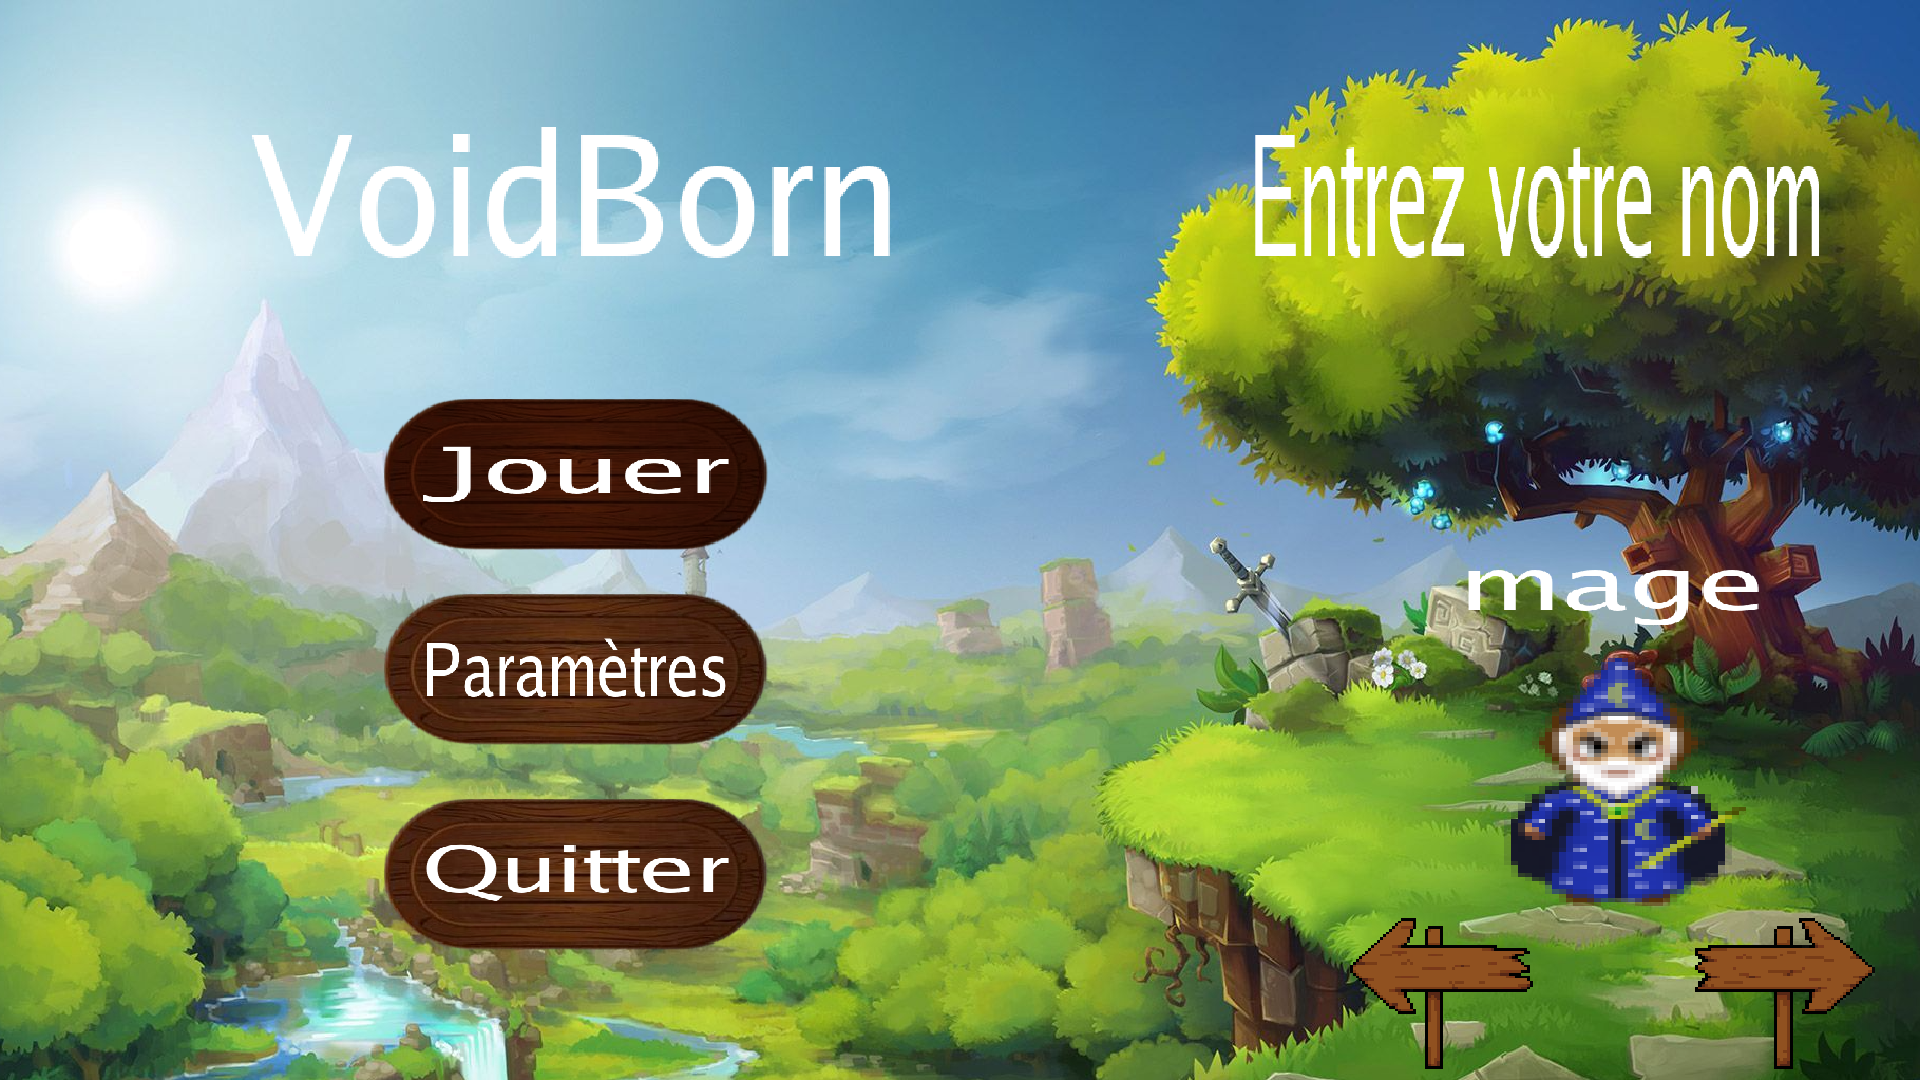
\includegraphics[height=6cm]{screenMenu.png}
                    \caption{Image menu principal lors du lancement du jeu}
                    \label{fig:mainMenu} 
                \end{center}
            \end{figure}
                \paragraph{Fonctionnalités du menu}
                Dès qu’il est lancé, une musique de fond se lance. Le menu renvoie un entier qui peut être :
                \begin{itemize}
                    \item-1 : quitter le menu sans jouer
                    \item 0 : rejoindre une partie créée par une autre personne en saisissant son adresse IP
                    \item 1 : être joueur et serveur à la fois
                    \item 2 : être uniquement serveur de la partie
                \end{itemize}
                Dans la page d’accueil du menu, il est possible de saisir son pseudo et de changer la classe de son personnage. Il est également possible de quitter le jeu directement sans le lancer ni être serveur. En cliquant sur l’onglet paramètres, une nouvelle section s’ouvre.\\ 
                Nous y trouvons : 
                \begin{itemize}
                    \item un bouton de retour au menu d’accueil,
                    \item un bouton de sauvegarde des paramètres,
                    \item un bouton charger_paramètres qui charge les paramètres dans ce même fichier,
                    \item un bouton plus et un bouton moins qui changent la valeur du volume de la musique du menu.
                \end{itemize}
   
                \paragraph{Affichage général}\leavevmode\newline
                Le menu peut être dans différents états représentés par un type enum pos\_actuelle. Cet enum est mis à jour en fonction des boutons cliqués par le joueur.  \\
                La fonction aff\_menu permet d’afficher la bonne partie du menu en fonction de la valeur de l’enum. 
                                
                \paragraph{Images}\leavevmode\newline
                Plusieurs images sont présentes dans le menu. On y retrouve différentes catégories : 
                \begin{itemize}
                    \item Personnages : les personnages disponibles pouvant être sélectionnés par le joueur
                    \item Boutons : les boutons principaux du menu sont des images utilisant un style boisé
                    \item Arrière-plan : une image dans le thème de la nature 
                \end{itemize}
                \leavevmode\newline
                Les images des personnages vus de face sont chargées en fonction du personnage sélectionné par le joueur. 
                Toutes les images chargées sont stockées dans un tableau de structures img\_t. Chaque structure possède deux champs : une \texttt{SDL\_Texture}\footnote{image ou surface graphique que l’on peut afficher à l’écran à l’aide de la fonction SDL\_Render\_Copy.} et la position de l’image représentée par un \texttt{SDL\_Rect}\footnote{structure de SDL à 4 champs : (coordonnées x et y de départ, longueur et largeur de la zone ou sera affichée l’image).}.\\
                Nous utilisons principalement quatre images de boutons boisés pour servir d’arrière-plan aux textes présents.

                \paragraph{Textes}\leavevmode\newline
                Les textes sont quant à eux chargés et sauvegardés dans un tableau de structures \textit{texte\_t} qui contient les mêmes champs que \textit{img\_t}, avec en plus un char* correspondant au texte affiché.\\
                À la création d’un texte, nous utilisons une police importée (Go-Regular), créons une \textit{SDL\_texture} et mettons le nouveau texte dans le  champ contenu.\\
                Certains textes doivent être modifiés dynamiquement. On utilise donc une fonction \textit{maj\_texte} qui recrée la texture si l’ancien texte est différent du nouveau.
                
                \begin{figure}[H]
                    \centering
                    % Première image
                    \begin{minipage}{0.45\textwidth}
                        \centering
                        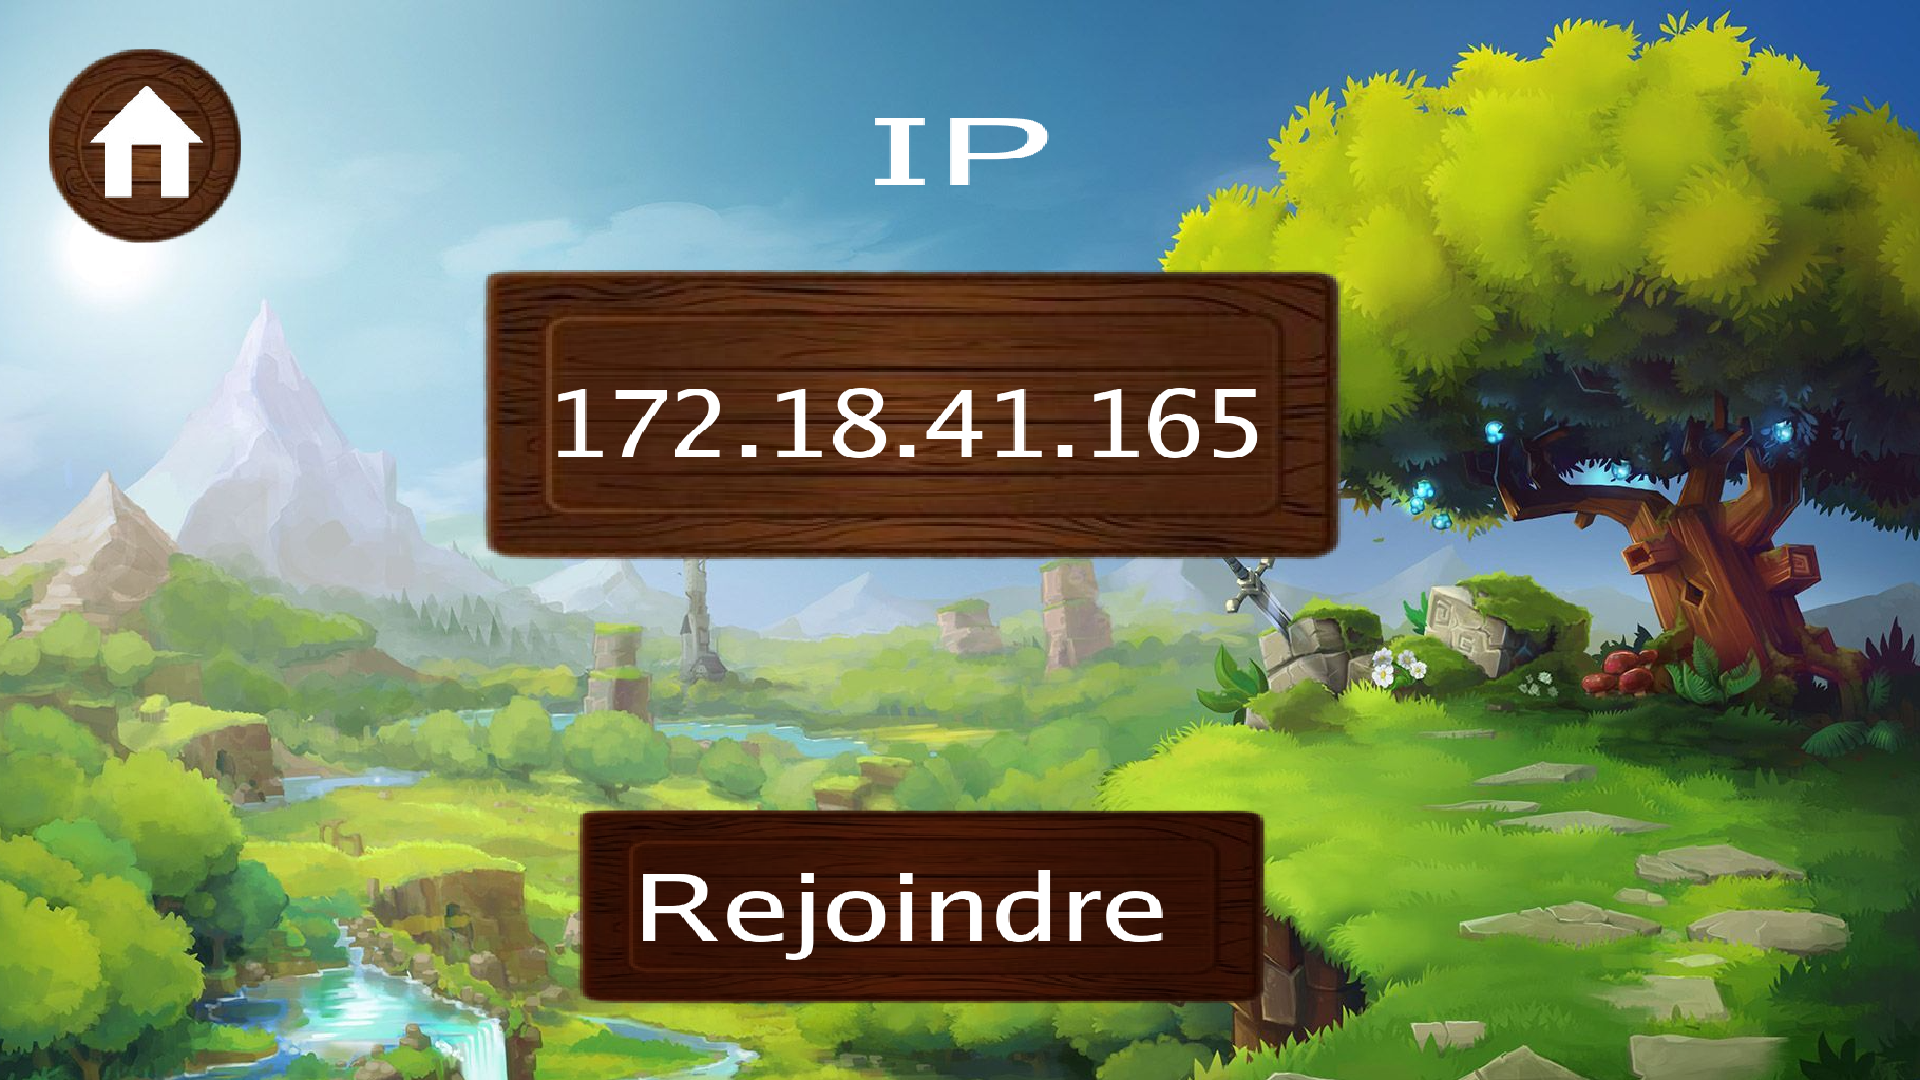
\includegraphics[height=3.6cm]{screenIpOk.png}
                        \caption{Affichage lorsque l'IP est valide}
                        \label{fig:IPOK}
                    \end{minipage}
                    \hfill
                    % Deuxième image
                    \begin{minipage}{0.45\textwidth}
                        \centering
                        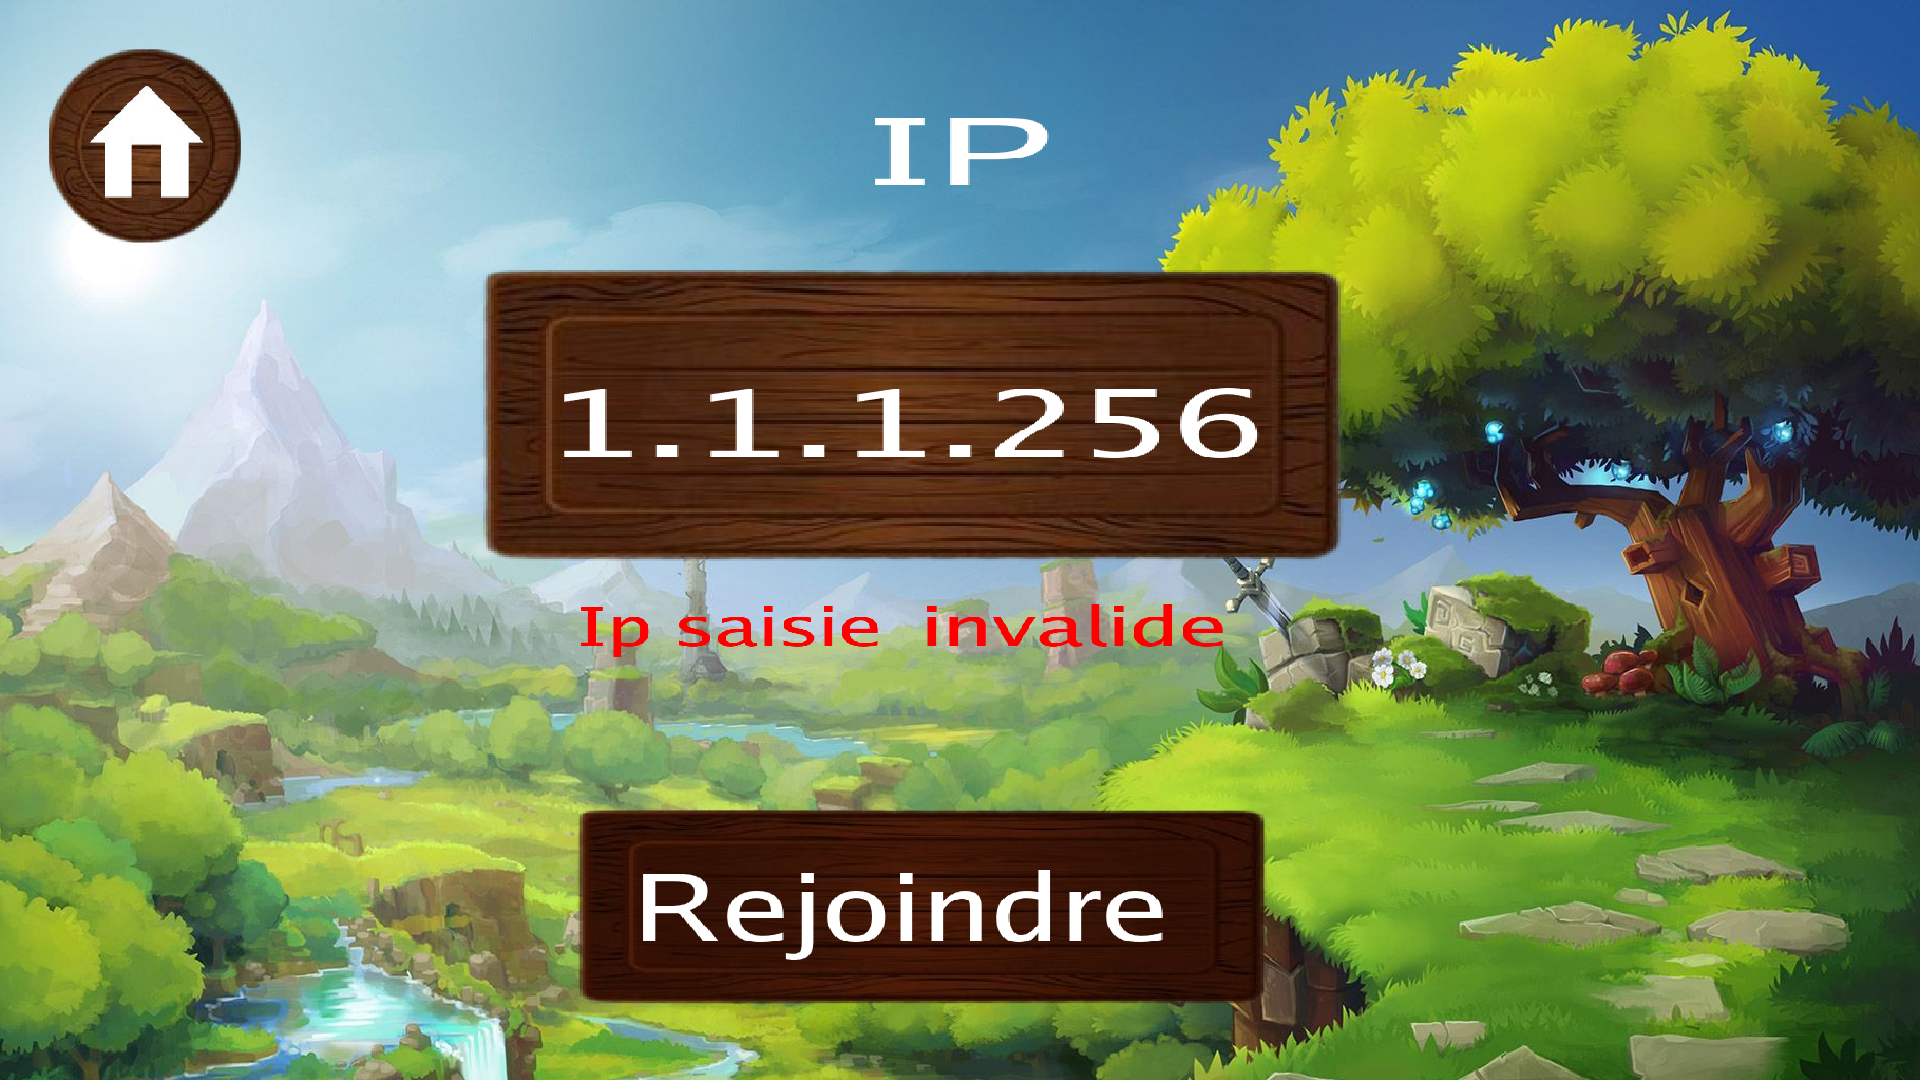
\includegraphics[height=3.6cm]{screenIpKo.png}
                        \caption{Affichage lorsque l'IP est invalide}
                        \label{fig:IPKO}
                    \end{minipage}
                \end{figure}
                \paragraph{Gestion des événements du menu}\leavevmode\newline
                Les événements en SDL sont gérés à l’aide d’une structure \textit{SDL\_Event} fournie par SDL. Nous nous en servons dans notre projet pour détecter les clics de la souris et les touches pressées au clavier. 

                    \subparagraph{souris}\leavevmode\newline
                    Les clics souris sont assez simples à gérer : si l’événement est de type clic de souris, on crée un \textit{\texttt{SDL\_Point}\footnote{une position sur la fenêtre représentée par deux coordonnées x et y.}} correspondant aux coordonnées du curseur de la souris. De nombreuses conditions testent si le clic de la souris est inclus dans le rectangle d’un bouton à l’aide de la fonction \textit{SDL\_PointInRect} et de la valeur de \textit{pos\_actuelle}. En fonction des boutons cliqués, différentes actions se passent. Il est possible de naviguer entre les différentes sections du menu de cette manière. 

                    \subparagraph{clavier}\leavevmode\newline
                    Les saisies au clavier servent à modifier des chaînes de caractères (adresse IP, pseudo du joueur) mais aussi à se déplacer dans les sections du mens à l’aide des flèches et des touches frappées. La saisie de l’adresse IP se fait via un switch dans la fonction \textit{saisie\_touche\_ip} vue précédemment. \\
                    Pour la saisie du nom du joueur, on ajoute simplement chaque caractère alphanumérique à la chaîne du nom du joueur. \\
                    Il est possible de supprimer les caractères dans les deux saisies.\\
                    
                    \begin{figure}[H]
                        \centering
                        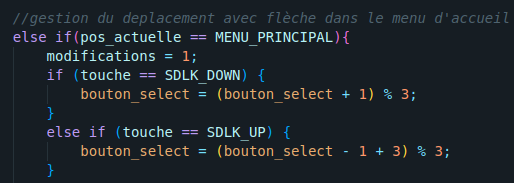
\includegraphics[height=5cm]{codeMenu.png}
                        \caption{voici un exemple de la gestion des déplacemen ts dans le menu via les flèches}
                        \label{fig:codeMenu}
                    \end{figure}
                    Si l’événement SDL est de type \textit{SDL\_KEYDOWN}, on crée un \textit{SDL\_Point} qui correspond aux coordonnées du bouton. \\
                    Lorsque l’on appuie sur la touche echap, cela force l’arrêt du menu.





            \subsubsection{Jeu}
            Dans cette partie, nous présenterons les moyens d’affichage des différents composants du jeu.\\\\
            Dans le jeu, le rendu de la map est généré en plusieurs étapes. Premièrement, la fonction \textit{init\_biomes} charge toutes les textures du jeu
            qui composent les tuiles (voir Figure~\ref{fig:normal}, ~\ref{fig:obstacle1}, ~\ref{fig:obstacle2} et ~\ref{fig:sortie}). Ensuite, les fonctions \textit{init\_map} et \textit{init\_tuile} génèrent pour chaque tuile une instance d’un biome. Enfin, il reste la phase d’exploitation : 
            quand un joueur entre sur une tuile. La fonction charger\_tuile s’occupe de créer le rendu qui sera affiché sur l’écran (qui est fixe) 
            à partir de la matrice de la tuile (voir exemple biome Figure \ref{fig:foret} et \ref{fig:glace}).
            Dans la boucle du jeu, cette texture est affichée avant les autres éléments du jeu à l’écran, graĉe à la bibliothèque SDL, car elle est le décor.\\
            \begin{figure}[H]
                \centering
                % Première image
                \begin{minipage}{0.45\textwidth}
                    \centering
                    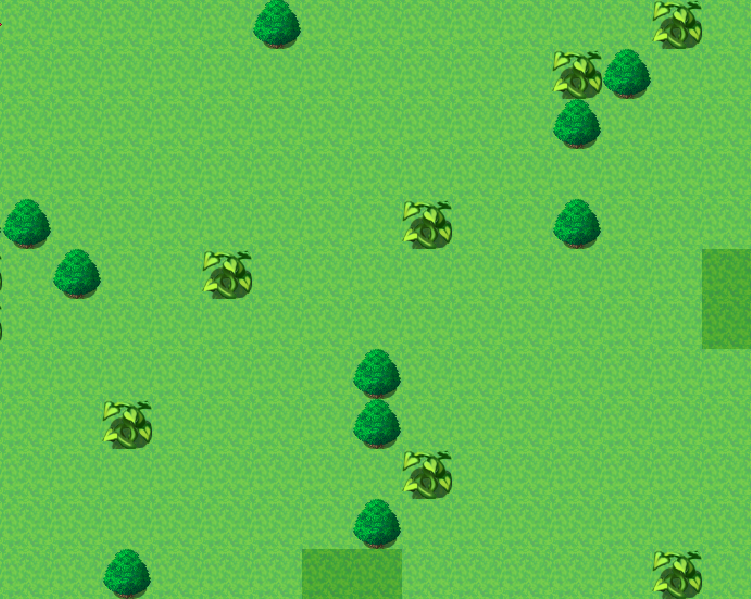
\includegraphics[height=5.5cm]{biomeForet.png}
                    \caption{Biome Forêt}
                    \label{fig:foret}
                \end{minipage}
                \hfill
                % Deuxième image
                \begin{minipage}{0.45\textwidth}
                    \centering
                    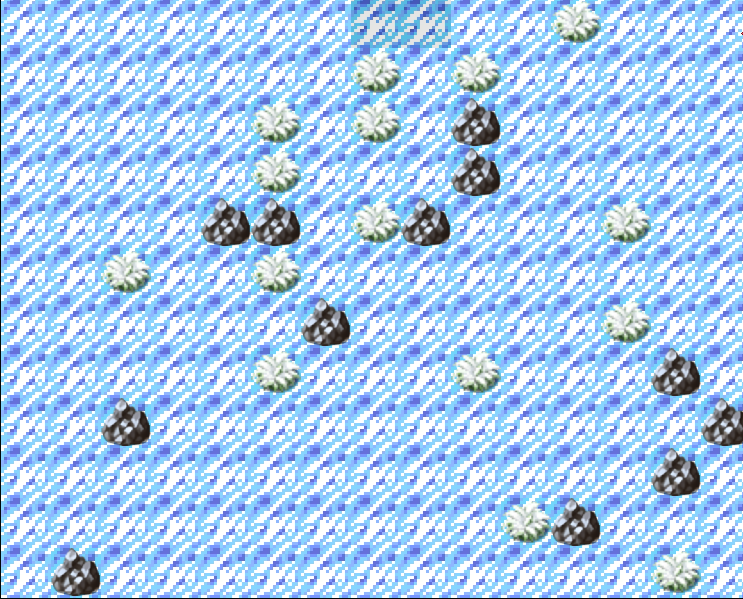
\includegraphics[height=5.5cm]{biomeGlace.png}
                    \caption{Biome glace}
                    \label{fig:glace}
                \end{minipage}
            \end{figure}
            Pour l’affichage des personnages. Nous avons développé une fonction \textit{charger\_sdl\_joueurs}, qui prend en paramètres le tableau des joueurs et un tableau 
            à deux dimensions qui stocke les différentes textures des personnages pour chaque direction. La fonction s’occupe de charger les bonnes images en fonction de la classe de chaque joueur. 
            Dans la boucle principale du client, la liste des personnages présents est parcourue, on affiche alors la texture du personnage qui correspond à sa direction, 
            à sa position courante.\\
            L’affichage des objets est similaire, les textures sont préchargées, puis, graĉe à la liste qui tient compte de ceux qui sont présents sur la même tuile 
            que le joueur, ils sont affichés.\\
            Les fonctions de destruction et de libération des ressources sont appelées à la fin du programme. 
            Les textures des objets, personnages, biomes doivent être détruites par la fonction SDL adéquate. 
            Tous les éléments des listes de chaque tuile sont aussi supprimés par \textit{detruire\_tuile}, faisant appel à \textit{detruire\_liste}.

                
    \section{Résultats et conclusion}
    L’état final du jeu rendu n’est pas conforme à nos premières attentes. De nombreuses fonctionnalités n’ont pas pu être ajoutées : les quêtes, l’ajout complet des objets dans le jeu (l’envoi des informations nécessaires entre le serveur et les clients est codé mais ils n’impactent pas le jeu) et l’implémentation des compétences des personnages (malgré la présence des bases pour le faire également). Cependant, les fonctionnalités les plus importantes sont réussies : la discussion entre les clients et le serveur permet aux joueurs de se rencontrer dans le jeu, les tuiles et la map sont réussies au niveau graphique, tout comme les personnages.\\
    Le planning prévisionnel n’a pas été respecté car nous avons abandonné de multiples fonctionnalités, mais celles qui ont été réalisées ont généralement suivi les dates imposées.\\
    Le développement du serveur et du client ont finalement duré du début à la fin du développement, il fallait les développer en parallèle des autres fonctionnalités car elles y sont toutes intégrées. La partie qui a le plus dépassé les prévisions était la gestion des collisions avec les obstacles de la map.\\
    Si nous avions un peu plus de temps pour améliorer le jeu, nous nous concentrerions sur le système de combat pour permettre la victoire d’une des équipes et développer les compétences, dont l’implémentation dans le code était en voie, pour que le jeu soit plus intéressant.
    

    \newpage
    \section{Annexes}
        \subsection{Débogage}
        
        \begin{figure}[H]
            \centering
            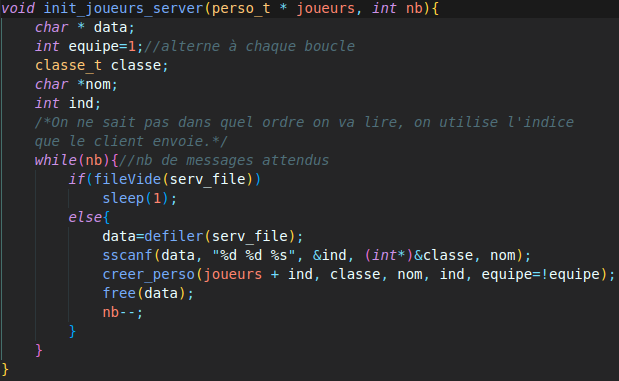
\includegraphics[height=7cm]{fonction.png}
            \caption{Fonction à tester}
            \label{fig:Mob}
        \end{figure}
        \begin{figure}[H]
            \centering
            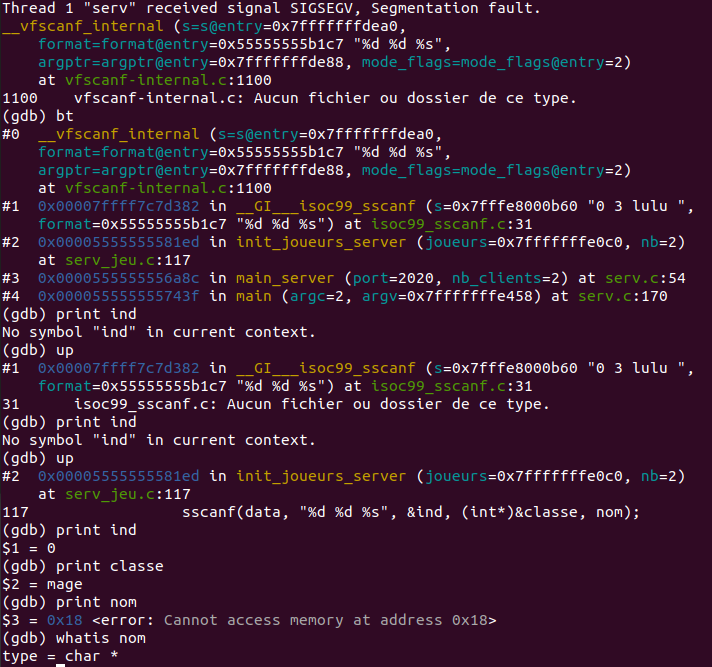
\includegraphics[height=10cm]{gdb.png}
            \caption{\textit{nom} ne doit pas être un pointeur mais un tableau alloué avec une taille fixe suffisante}
        \end{figure}


\end{document}
